%!TEX root = main.tex
\section{Characterizing Synchronous Traces}

We give a characterization of the traces generated by the $k$-synchronous semantics that uses a notion of \emph{conflict-graph} similar to the one used in conflict serializability~\cite{journals/jacm/Papadimitriou79b}. The nodes of the conflict graph correspond to pairs of matching actions (a send and a receive) or to unmatched sends, and the edges represent the program order relation between the actions represented by these nodes. For instance, an execution for which the conflict graph of its trace is acyclic, e.g., the execution in Figure~\ref{fig:commit-exec}, is ``equivalent'' to an execution where every receive immediately follows the matching send. Ignoring unmatched sends, such an execution can be obtained using rendez-vous communication. In general, it is an execution of the $1$-synchronous semantics. For arbitrary values of $k$, the conflict graph may contain cycles, but of a particular form. For instance, traces of the $2$-synchronous semantics may contain a cycle of size 2 like the one in Figure~\ref{fig:elevator-exec}(b). More generally, we show that the conflict graph of a $k$-synchronous trace cannot contain cycles of size strictly bigger than $k$. However, this class of cycles is not sufficient to characterize precisely the $k$-synchronous traces. Consider for instance the trace on the left of Figure~\ref{fig:ex-rs-cycle}. The conflict-graph of this trace contains a cycle of size $4$ (shown on the right), but the trace is not $4$-synchronous. The reason is that the messages tagged by $1$ and $4$ must be sent during the same exchange transition, but receiving message $4$ needs that the message $3$ is sent after $2$ is received. Therefore, it is not possible to schedule all the send actions before all the receives. Such scenarios correspond to cycles in the conflict graph where at least one receive is before a send in the program order. We show that excluding such cycles, in addition to cycles of size strictly bigger than $k$, is a precise characterization of $k$-synchronous traces.

\begin{figure}[t]
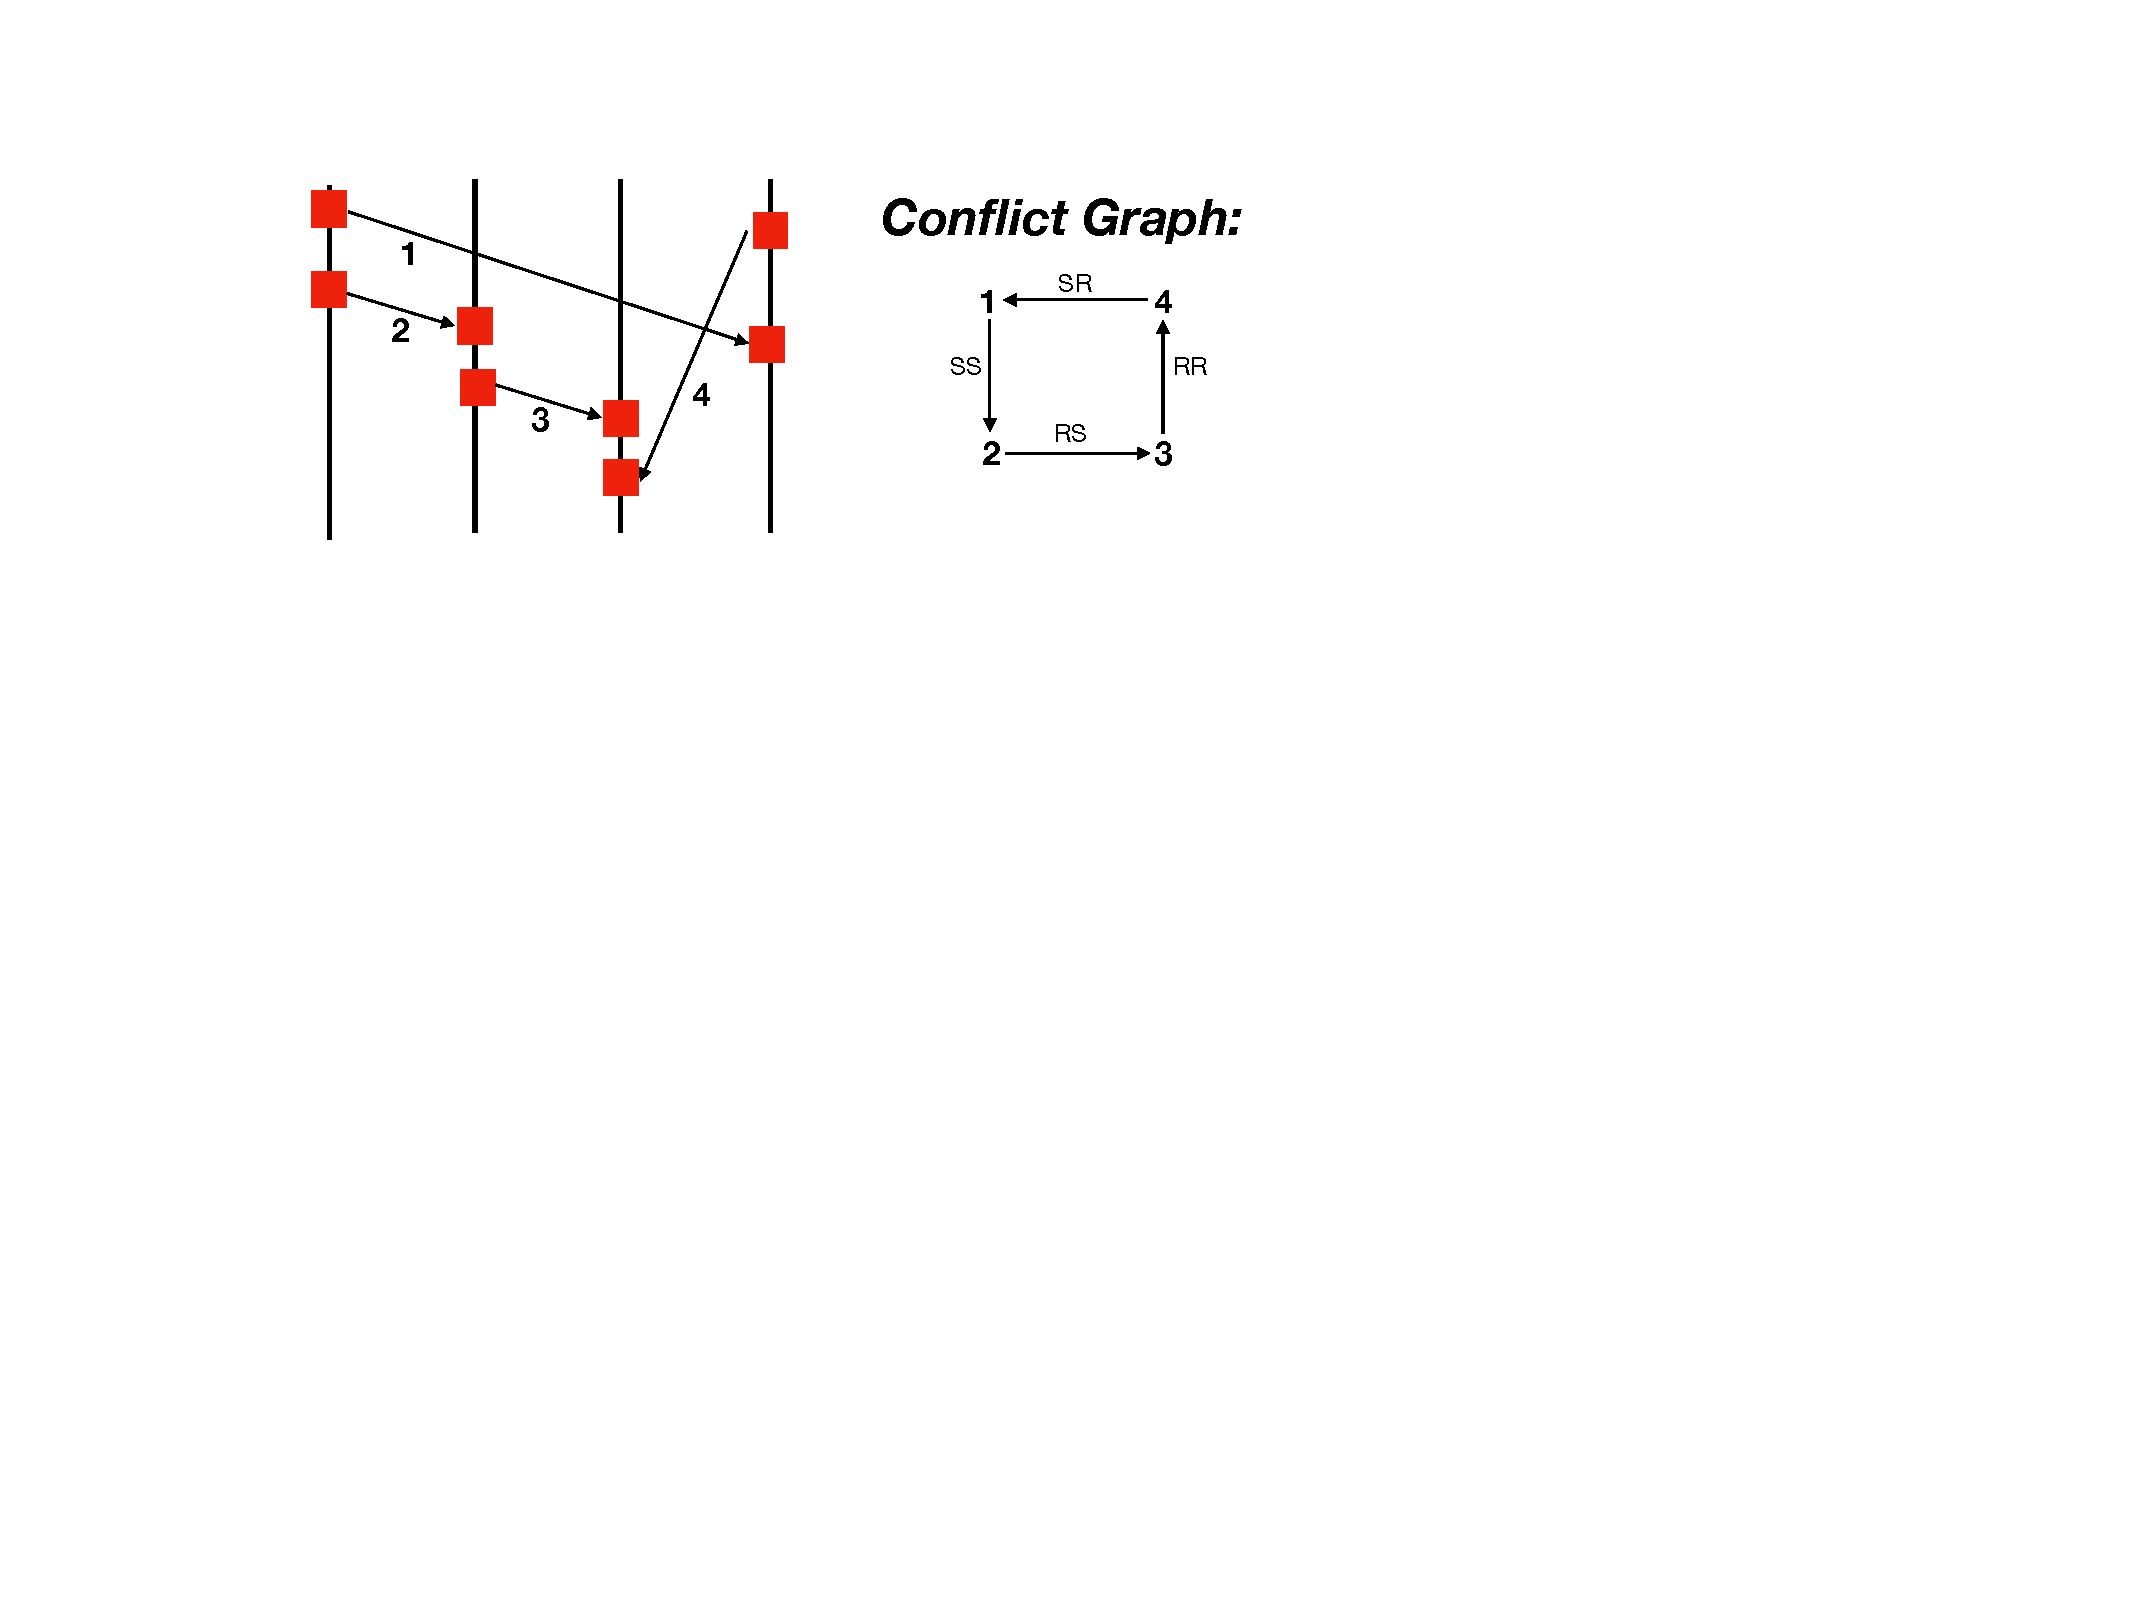
\includegraphics[width=6cm]{ex-rs-cycle.pdf}
\caption{A trace which is not $k$-synchronous, for every $k$.}
\label{fig:ex-rs-cycle}
\end{figure}

%define a notion of robustness, called \emph{synchronizability}, which ensures that even if the system uses buffers to store messages it provides the illusion that messages are received instantaneously, as in a synchronous (rendez-vous) semantics. This is analogous to the atomicity criterion for concurrent shared-memory systems, where even though transactions can interleave, every execution is “equivalent” to an execution where transactions happen atomically without interference.

%\subsection{Defining Robustness}


%\begin{lemma}
%For a given trace $t$, $\asynchTr{A}$ contains every conflict-preserving permutation $t'$ of $t$ when $t\in \asynchTr{A}$.
%\end{lemma}
%
%A trace $t$ is called \emph{synchronous} when every send $s\in S_{id}$ is immediately followed by the matching receive. Formally, for every $0\leq k< |t| -1$, if $t_k\in S_{id}$ then $t_{k+1}\in R_{id}$ and $t_{k}\match t_{k+1}$.

%Informally, a trace  $t$ is called \emph{synchronizable} when there exists a conflict-preserving permutation of $t$ which is synchronous.
%The presence of unmatched send actions introduces a subtlety: a trace is considered synchronizable by supposing that every message is eventually received.
%To account for this, we define a \emph{completion} of a trace $t$ to be any sequence $t\cdot t'$ where $t'$ contains only receive actions that match one of the unmatched send actions in $t$.
%
%\begin{definition}
%A trace $t$ is called \emph{synchronizable} when there exists a synchronous conflict-preserving permutation of a completion of $t$. 
%\end{definition}





%A message passing system $A$ is synchronizable when every trace $t\in \asynchTr{A}$ is  synchronizable.

%\begin{figure} [t]
%\footnotesize{
%  \centering
%  \begin{mathpar}
%    \inferrule[send]{
%      l\in \delta(\vec{l}_p,\senda{p,q,v}) \neq \emptyset \\
%      \mathrm{empty}(\vec{b}_j) \mbox{ for all $j$} 
%    }{
%      \vec{l},\vec{b}
%      \xRightarrow{\senda{p,q,v}}
%      \vec{l}[\vec{l}_p\gets l],\vec{b}[\vec{b}_q.\ \mathrm{add}(v)]
%    }%\hspace{5mm}
%
%%    \inferrule[orphan send]{
%%      m= \tup{i,j,p} \\
%%      \delta(\vec{l}_i,\send{i}{m})\neq \emptyset
%%    }{
%%      \vec{l},\vec{b}
%%      \xRightarrow{\send{i}{m}}
%%      \vec{l}[\vec{l_i}\gets \delta(\vec{l}_i,\send{i}{m})],\vec{b}
%%    }%\hspace{5mm}
%    
%        \inferrule[local]{ 
%      l \in \delta(\vec{l}_p,\epsilon) \neq \emptyset
%    }{
%      \vec{l},\vec{b}
%      \xrightarrow{\epsilon}
%      \vec{l}[\vec{l}_p\gets l],\vec{b}
%    }%\hspace{5mm}
%    
%    \inferrule[receive]{
%      v = \vec{b}_q.\ \mathrm{rem}() \\
%      l\in \delta(\vec{l}_q,\reca{q,v}) \neq \emptyset \\
%      \mathrm{empty}(\vec{b}_j) \mbox{ for all $j\neq q$} 
%    }{
%      \vec{l},\vec{b}
%      \xRightarrow{\reca{q,v}}
%      \vec{l}[\vec{l}_q\gets l],\vec{b}[\vec{b}_q.\ \mathrm{rem}()]
%    }%\hspace{5mm}
%  \end{mathpar}
%  }
%% \vspace{-5mm}
%  \caption{The synchronous semantics of a message passing system $A$. The predicate $\mathrm{empty}(\vec{b}_j)$ denotes the fact that the buffer $\vec{b}_j$ is empty, i.e, $\vec{b}_j.\ \mathrm{rem}()$ is not enabled.}
%  \label{fig:synch-sem}
%%\vspace{-6mm}
%\end{figure}
%
%The transition relation $\Rightarrow$ in Figure~\ref{fig:asynch-sem} defines a new semantics for  a message passing system $A$
%where a receive action of a process $q$ is enabled only if the buffers of all the other processes are empty and the buffer of process $q$
%contains exactly one message. Executions and reachable local
%state vectors under the new semantics, denoted by $\synch{States}(A)$, are defined as in Section~\ref{sec:prelims}.
%The set of traces of $A$ under the new semantics is denoted by $\synch{Tr}(A)$.
%
%TODO DESCRIBE TRANSITIONS 
%
%\begin{lemma}\label{lem:sync_traces}
%The synchronous semantics of a message passing system $A$ admits every synchronous trace of $A$ under the asynchronous semantics.
%\end{lemma}
%
%TODO DEFINE THE CONDITION XXX THAT EVERY MESSAGE IS EVENTUALLY RECEIVED



%\section{Monitoring Synchronizability}\label{sec:monitoring}

%\begin{example}
%The traces in Example~\ref{ex:perm} are $1$-synchronizable while the following are not:
%\begin{align*}
%\send{1}{p,q,\_}\ 
%\send{2}{p,q,\_}\ 
%\rec{2}{q,\_}\ 
%\rec{1}{q,\_} \\
%\send{1}{p,q,\_}\ 
%\send{2}{q,p,\_}\ 
%\rec{2}{p,\_}\ 
%\rec{1}{q,\_} \\
%\send{1}{p,q,\_}\ 
%\send{2}{q,p,\_}\ 
%\end{align*}
%
%The latter trace demonstrates the use of completions in defining synchronizability: none of its completions, i.e., one of the first two traces, cannot be permuted to a synchronous trace.
%\end{example}


%Checking that a given trace is synchronizable can be done by tracking a ``conflict-graph'' like in conflict serializability~\cite{}
%to show that every pair of matching send and receive actions can be executed atomically. Roughly, the nodes of this graph
%correspond to such pairs of matching actions, and the edges to conflicts between actions from one pair and another. 
%Then, a trace is synchronizable if{f} the conflict-graph is acyclic. Dealing with unmatched sends and completions 
%poses a technical difficulty since the conflict-graph should contain enough additional edges
%to anticipate for the possible completions. 
%
%Before defining conflict-graphs, we define a notion of action-graph that represents the order between all conflicting actions in some given trace.
%
%\begin{definition}[Action-Graph]\label{def:pr_graphs}
%    The \emph{action-graph} of a trace $t$ is the directed graph 
%    $G_t = \tup{V,E}$ where there is a node in $V$ for each action in $t$, and $E$ 
%    contains an edge from $u$ to $v$ iff $\mathrm{act}(u) \prec \mathrm{act}(v)$ and $\mathrm{act}(u)$ occurs before $\mathrm{act}(v)$ in $t$ (where $\mathrm{act}(v)$ is the action of trace $t$ corresponding to the graph node $v$).
%\end{definition}
%%Intuitively, one can think of the action-graph of a trace $t$ as a structure that represents the order between all conflicting actions in $t$.
%%AND THE WEAKEST CONSTRAINTS THAT CAN BE ADDED BY A COMPLETION.
%For two actions $a$ and $a'$ in a trace $t$, $a\leadsto a'$ denotes the fact that $G_t$ contains a path from the node representing $a$ to that representing $a'$.
%
%\begin{lemma}\label{lem:acyclic_ag}
%	The \emph{action-graph} of a trace is acyclic. 
%%	Moreover, $\rec{1}{q_1,\_}\leadsto \send{2}{p_2,q_2,\_}$ and $\rec{2}{q_2,\_}\leadsto \send{1}{p_1,q_1,\_}$ is impossible for any possible instantiation of $p_1$, $q_1$, $p_2$, and $q_2$.
%\end{lemma}

%TODO BELOW WE ADD EDGES FROM A SEND/RECEIVE PAIR TO EVERY UNMATCHED SEND THAT HAS THE SAME DESTINATION

\begin{definition}[Conflict-Graph]\label{def:conf_graph}
    The \emph{conflict-graph} of a trace $t=(A,po,src)$ is the labeled directed graph $CG_t=\tup{V,E,\ell_E}$ where:
\begin{itemize}
	\item the set of nodes $V$ includes one node for each pair of matching send and receive actions, and each unmatched send action in $t$. 
	%Nodes $v$ corresponding to pairs of send/receive actions are labeled by $M$, i.e., $\ell_V(v)=M$, and those corresponding to unmatched sends by $U$, i.e., $\ell_V(v)=U$.
    	\item the set of edges $E$ is defined by: $(v,v') \in E'$ iff there exist actions $a \in \mathrm{act}(v)$ and $a' \in \mathrm{act}(v')$ such that $(a,a') \in po$ (where $\mathrm{act}(v)$ is the set of actions of trace $t$ corresponding to the graph node $v$). The label of the edge $(v,v')$ records whether $a$ and $a'$ are send or receive actions, i.e., for all $X,Y\in \{S,R\}$, $XY\in \ell(v,v')$ iff $a\in X_{id}$ and $a'\in Y_{id}$.
\end{itemize}
\end{definition}

A direct consequence of previous results on conflict serializability~\cite{journals/jacm/Papadimitriou79b} is that 
a trace is $1$-synchronous whenever its conflict-graph is acyclic.

\begin{lemma}\label{lem:cg_1}
A trace $t$ is $1$-synchronous if{f} its conflict-graph is acyclic.
\end{lemma}

A cycle of a conflict graph $CG_t$ is called \emph{bad} when it contains %a node labeled by $U$, or 
an edge labeled by $RS$.
%or it is formed of two edges, one labeled by $SS$ and one by $RR$. 
Otherwise, it is called \emph{good}.
The following extends Lemma~\ref{lem:cg_1} to $k$-synchronous traces.

%TODO IN THE FOLLOWING I'M ASSUMING THAT THE TRACE COMES FROM THE FIFO SEMANTICS (SO $S_1 S_2 R_2$ CAN'T HAPPEN). 

\begin{theorem}\label{lem:cg_k}
A trace $t$ satisfying causal delivery is $k$-synchronous if{f} every cycle in its conflict-graph is good and of size at most $k$.
\end{theorem}
\begin{proof}
For the only if direction, $t$ is the trace of an execution $e\in \synchExec{\mathcal{S}}{k}$ for some system $\mathcal{S}$. The execution $e$ is obtained through a sequence of \textsc{$k$-exchange} transitions. The set of actions of every node $v$ of $CG_t$ appear in the label of a single such transition. Moreover, for every cycle in $CG_t$, the actions corresponding to the nodes in this cycle occur in the label of a single \textsc{$k$-exchange} transition. Therefore, every cycle in $CG_t$ is good and of size at most $k$.

For the if direction, we first show that any strongly-connected component $C$ of $CG_t$ is $k$-synchronous. Since all the cycles in $CG_t$ are of size at most $k$, we get that $C$ contains at most $k$ nodes. The case of strongly-connected components formed of a single node $v$ is trivial. The actions corresponding to $v$ are either a matching pair of send/receive actions, which can be generated through a \textsc{$1$-exchange} transition, or an unmatched send, which can also be generated through a \textsc{$1$-exchange} transition. Now, let $C$ be formed of a set of nodes 
$v_1$,$\ldots$, $v_n$, for some $2\leq n\leq k$ such that $s_i\in act(v_i)$, for all $1\leq i\leq n$. 
W.l.o.g., assume that the indexing of the nodes in $C$ is consistent with the edges labeled by SS (note that there is no cycle formed only of edges labeled by SS), i.e., for every $1\leq i_1<i_2\leq n$, $C$ doesn't contain an edge labeled by SS from $i_2$ to $i_1$, and for every $1\leq i_1<i_2<i_3\leq n$, if $\<proc>(s_{i_1})=\<proc>(s_{i_3})$, then $\<proc>(s_{i_1})=\<proc>(s_{i_2})$. Let $i_1$,$\ldots$,$i_m$ be the maximal subsequence of $1$,$\ldots$,$n$ such that $r_{i_j}\in act(v_i)$ for every $1\leq j\leq m$. 
We have that $C$ is the trace of the execution $e=s_1\cdot\ldots\cdot s_n\cdot r_{i_1}\cdot\ldots\cdot r_{i_m}$. The fact that all sends can be executed before the receives is a consequence of the fact that $C$ doesn't contain edges labeled by $RS$. Then, the order between receives is consistent with the one between sends because $C$ satisfies causal delivery. By definition, $e$ is the label of an \textsc{$n$-exchange} transition, and therefore, $C$ is $k$-synchronous. 

To complete the proof we proceed by induction on the number of strongly connected components of $CG_t$. The base case is trivial. 
 For the induction step, assume that the claim holds for every trace whose conflict-graph has at most $n$ strongly connected components, and 
 let $t$ be a trace with $n+1$ strongly connected components.  
 Let $C$ be a strongly connected component of $t$ such that
% \begin{itemize}
% 	\item 
$C$ has no outgoing edges towards another strongly connected component of $t$.
%	\item $C$ doesn't contain a receive action $\rec{i}{q,v}$ such that one of the other $n$ strongly connected components contains an unmatched send action $\send{j}{p',q,v'}$ (executing this send before the actions in $C$ would not be possible under the synchronous semantics).
%\end{itemize}
%It is possible to chose such a strongly connected component because $t$ satisfies causal delivery.
%
 By the definition of the conflict-graph, $t$ is the trace of an execution $e=e'\cdot e''$ where $e''$ contains all the actions corresponding to the nodes of $C$. 
 We have shown above that $e''$ is $k$-synchronous, and by the induction hypothesis, $e'$ is also $k$-synchronous. Therefore, $e$ is $k$-synchronous.
\end{proof}

Theorem~\ref{lem:cg_k} can be used to define a runtime monitor checking for $k$-synchronizability. 
The monitor maintains the conflict-graph of the trace produced by the message passing system and checks whether it contains some bad cycle, or a cycle of size bigger than $k$.
While this approach requires dealing with the complexity of the asynchronous semantics (the unbounded message buffers), the next section shows that this is not necessary. Synchronizability violations, if any, can be exposed by executing the system under the \emph{synchronous} semantics.




